\documentclass[12pt, oneside, titlepage]{article}   	% use "amsart" instead of "article" for AMSLaTeX format

\setlength{\parindent}{5ex}

\usepackage{graphicx}
\graphicspath{ {\string} }
\usepackage{subcaption}

%%%%%%%%%%%%%%%%%%%%%%%%%%%%%%%%%%%%%%%%%%%%%%%%%%%%
% tables
%%%%%%%%%%%%%%%%%%%%%%%%%%%%%%%%%%%%%%%%%%%%%%%%%%%%
\usepackage{bm}   
\usepackage{tabularx}   

\usepackage{caption}          
 \captionsetup[table]{labelfont=sc}

\usepackage{amsmath}                      
\usepackage{amssymb}      

%%%%%%%%%%%%%%%%%%%%%%%%%%%%%%%%%%%%%%%%%%%%%%%%%%%%
% set up packages
%%%%%%%%%%%%%%%%%%%%%%%%%%%%%%%%%%%%%%%%%%%%%%%%%%%%
\usepackage{geometry}                
\usepackage{textcomp}                
\usepackage{amsmath}                
\usepackage{graphicx}                
\usepackage{amssymb}                
\usepackage{fancyhdr}                
\usepackage{subcaption}                
\usepackage{bm}                
\usepackage{lineno}
% package for comments
\usepackage{soul}
\usepackage[usenames, dvipsnames]{color}

\usepackage[breaklinks=true]{hyperref}
\hypersetup{
    colorlinks=true,
    linkcolor=red,
    filecolor=orange,      
    urlcolor=red,
    citecolor=Violet,
}

\usepackage[superscript,noadjust]{cite} % puts dash in citations to abbreviate
\usepackage [autostyle, english = american]{csquotes} % sets US-style quotes

\usepackage{etoolbox} % block quotes

\usepackage{float}

\usepackage{pgf}
\usepackage{tikz}
\usepackage{eqnarray}

\usepackage{listings} % code blocks
\usepackage{setspace}

\usepackage{natbib}
%\bibliographystyle{abbrvnat}
\setcitestyle{authoryear}

% Adds parentheses around year
%\setcitestyle{authoryear,open={(},close={)}}

%%%%%%%%%%%%%%%%%%%%%%%%%%%%%%%%%%%%%%%%%%%%%%%%%%%%
% call packages
%%%%%%%%%%%%%%%%%%%%%%%%%%%%%%%%%%%%%%%%%%%%%%%%%%%%	
\geometry{letterpaper, marginparwidth=60pt} % sets up geometry              		
\linenumbers % adds line numbers 
\MakeOuterQuote{"} % sets quote style
\doublespacing % setspace

%%%%%%%%%%%%%%%%%%%%%%%%%%%%%%%%%%%%%%%%%%%%%%%%%%%%
% patches with etoolbox 
%%%%%%%%%%%%%%%%%%%%%%%%%%%%%%%%%%%%%%%%%%%%%%%%%%%%	

% linenumbers
\makeatletter
\patchcmd{\@startsection}{\@ifstar}{\nolinenumbers\@ifstar}{}{}
\patchcmd{\@xsect}{\ignorespaces}{\linenumbers\ignorespaces}{}{}
\makeatother

%%%%%%%%%%%%%%%%%%%%%%%%%%%%%%%%%%%%%%%%%%%%%%%%%%%%
% page formatting; exact 1 in margins
%%%%%%%%%%%%%%%%%%%%%%%%%%%%%%%%%%%%%%%%%%%%%%%%%%%%
\pagestyle{plain}                                                     

\setlength{\textwidth}{6.5in}    
\setlength{\oddsidemargin}{0in}
\setlength{\evensidemargin}{0in}
\setlength{\textheight}{8.5in}
\setlength{\topmargin}{0in}
\setlength{\headheight}{0in}
\setlength{\headsep}{0in}
\setlength{\footskip}{.5in}

\usepackage{wrapfig}


%%%%%%%%%%%%%%%%%%%%%%%%%%%%%%%%%%%%%%%%%%%%%%%%%%%%
% TABLE OF CONTENTS TITLE
%%%%%%%%%%%%%%%%%%%%%%%%%%%%%%%%%%%%%%%%%%%%%%%%%%%%
\renewcommand{\contentsname}{Parameter estimation details}
\setcounter{tocdepth}{3}

%%%%%%%%%%%%%%%%%%%%%%%%%%%%%%%%%%%%%%%%%%%%%%%%%%%%
%%%%%%%%%%%%%%%%%%%%%%%%%%%%%%%%%%%%%%%%%%%%%%%%%%%%
% begin document
%%%%%%%%%%%%%%%%%%%%%%%%%%%%%%%%%%%%%%%%%%%%%%%%%%%%
%%%%%%%%%%%%%%%%%%%%%%%%%%%%%%%%%%%%%%%%%%%%%%%%%%%%

\begin{document}

\tableofcontents

\clearpage
%%%%%%%%%%%%%%%%%%%%%%%%%%%%%%%%%%%%%%%%%%%%%%%%%%%%
% METHODS
%%%%%%%%%%%%%%%%%%%%%%%%%%%%%%%%%%%%%%%%%%%%%%%%%%%%
%\section\subsection{Methods}

\section{Clarkia life history}

\textit{Clarkia xantiana} is a winter annual. \textit{C. xantiana} seeds germinate with late fall and winter rains; in the Kern Valley this is between October and late February or early March. Seedlings grow throughout the winter and spring, and surviving plants flower in late spring and early summer, April into early July. Pollinated fruits set seed in the early summer, June to July. Seeds of \textit{C. xantiana} are produced in early summer, with fruits that dry out and gradually split open. Most seeds appear to be shed from fruits within 3-4 months after production, but can remain on the plant for up to a year. Seeds are small ($<1$ mm in width) and have no structures to aid in aerial dispersal. Seeds can remain viable in the field and laboratory for at least 5 years, contrary to previous suggestions that seeds are unlikely to persist past a few years (\hl{Lewis 1962}). 

\begin{wrapfigure}[]{r}{0.5\textwidth}
       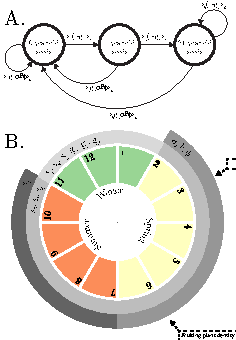
\includegraphics[scale=1.9]{../../manuscript/figures/model-figure.pdf}  
        \caption{ Diagram representations of Clarkia life cycle. }
        \label{fig:life-cycle}
\end{wrapfigure}

We represent the \textit{Clarkia xantiana} as a life cycle graph (Figure \ref{fig:life-cycle}A) that describes transitions from October of year $t$ to October of year $t+1$ in terms of underlying vital rates. The census period occurs when the entire population is seeds, and corresponds to the time at which seed bags are placed into the field (\hl{see below}). Seeds are grouped into three stages: age 0 seeds, which were produced in the current year; age 1 seeds, which were produced in the previous year; age 2+ seeds, which were produced two or more years ago. Persistence of seeds in the seed bank is represented by transitions from younger to older seeds. Production of new seeds is captured by transition to the age 0 seed state. 

Transitions in the life cycle graph are the product of age-specific seed survival and germination, and aboveground seedling survival to fruiting, fruit production, and seeds per fruit. Seed-related rates are represented separately for age 0, 1, and 2+ seeds. Germination for each age class is given as $g_1$, $g_2$, and $g_3$, respectively. Seed survival from seed production to the first October is given as $s_0$, and survival from October to February is given as $s_1$, $s_3$, and $s_5$ for age 0, 1, and 2+ seeds, respectively. Survival from February to October is given as $s_2$, $s_4$, and $s_6$ for age 0, 1, and 2+ seeds, respectively. We assume that vital rates remain unchanged after age 2. We also we assume that all plants experience the same vital rates upon germination seed age at germination does not affect seedling survival to fruiting ($\sigma$), fruits per plant ($F$), or seeds per fruit ($\phi$).

The life cycle graph (Figure \ref{fig:life-cycle}A) corresponds to the annual projection matrix
%
\begin{gather}
\bm{A} = 
\begin{bmatrix} 
s_1 g_1 \sigma F \phi s_0 & s_3 g_2 \sigma F \phi s_0 & s_5 g_3 \sigma F \phi s_0 \\
s_1 (1-g_1) s_2 & 0 & 0 \\
0 & s_3 (1-g_2) s_4  & s_5 (1-g_3) s_6  \\
\end{bmatrix}
\label{eq:projection-matrix}
\end{gather} 
%
that summarizes transitions between stages. 

\section{Creating the dataset}

We used field surveys and experiments to assemble the demographic observations necessary to provide insight into the population dynamics of \textit{Clarkia xantiana} (Table \ref{tab:datasets}). Specifically, we sought to parameterize the structured population model for \textit{Clarkia xantiana} populations represented by Equation \ref{eq:projection-matrix}. 

Starting in 2006, Monica Geber and collaborators collected annual estimates for demographic data on the winter annual plant \textit{Clarkia xantiana} ssp. \textit{xantiana}. The data include annual estimates for survival of seedlings to fruiting adults, fruits per adult plant, and seeds per fruit. In addition the data on above-ground vital rates, experiments have been used to infer germination and seed survival in the seed bank. The demographic study has been used to test hypotheses about the geography of demography (\hl{Eckhart et al. 2011}) and species distributions (\hl{Pironon et al. 2018}).

We used an experiment to estimate transitions in the seed bank. The experiment has been previously described in \hl{Eckhart et al. 2011} and we reanalyze the data here. From 2006-2009, Geber and collaborators buried seeds in bags and periodically dug them up to count seedlings and intact, viable seeds. This data estimates transitions leading to germination or survival of seeds that are 1, 2, and 3 years old.

Starting in 2007, there are (1) estimates of fruits/plant and seeds/fruit that provide an estimate of seed input into a plot and (2) estimates of germinants the following year. For most plots, the number of seeds entering a plot in year $t-1$ is much greater than the number of seedlings emerging in a plot in year $t$. However, this is not uniformly true, and there is also experimental data suggesting these seeds may survive in the seed bank for at least 10 years at some locations.

Key: experiments from 2006-2009 to estimate age-specific seed rates.

Field surveys in permanent plots to estimate seedling survival to fruiting.

Combine data from permanent plots and additional grids to estimate fruits per plant.

Collect fruits to estimate seeds per fruit. 

\begin{singlespace*}...
\captionof{table}{ Summary of data sets used to estimate parameters. } \label{tab:datasets} 
\begin{center}
%\documentclass[varwidth=\maxdimen,border=1pt]{standalone}
%                 
%\usepackage{bm}   
%\usepackage{tabularx}   
%
%\usepackage{caption}          
% \captionsetup[table]{labelfont=sc}
%
%\usepackage{amsmath}                      
%\usepackage{amssymb}      
%
%
%%%%%%%%%%%%%%%%%%%%%%%%%%%%%%%%%%%%%%%%%%%%%%%%%%%%%
%%%%%%%%%%%%%%%%%%%%%%%%%%%%%%%%%%%%%%%%%%%%%%%%%%%%%
%% begin document
%%%%%%%%%%%%%%%%%%%%%%%%%%%%%%%%%%%%%%%%%%%%%%%%%%%%%
%%%%%%%%%%%%%%%%%%%%%%%%%%%%%%%%%%%%%%%%%%%%%%%%%%%%%
%
%\begin{document}

%%%%%%%%%%%%%%%%%%%%%%%%%%%%%%%%%%
% DATASETS
%%%%%%%%%%%%%%%%%%%%%%%%%%%%%%%%%%

%\captionof{table}{ Summary of data sets used to estimate parameters. } \label{tab:title1} 
  \begin{tabularx}{\linewidth}{ l l c c } 
 \hline
 \hline
\multicolumn{1}{ c }{ Parameter data } & 
\multicolumn{1}{ c }{ Description } & 
\multicolumn{1}{ c }{ Data set }  & 
\multicolumn{1}{ c }{ Time span } \\
 \hline
 % seed bag burial experiment
 \textsc{Seed vital rates} & --- & --- & --- \\ 
 Seed survival and germination & Seed bag burial & $\bm{\mathrm{Y}}_1$ & 2006-2009  \\ 
 Seed viability & Viability trials & $\bm{\mathrm{Y}}_2$ & 2006-2009 \\ 
 Seed survival and germination & Seed pots & $\bm{\mathrm{Y}}_3$ & 2013-2019  \\ 
 \textsc{Seedling survival} & --- & --- & --- \\ 
 Seedling survival to fruiting & Field surveys & $\bm{\mathrm{Y}}_4$ & 2006-2019 \\ 
 \textsc{Fruits per plant} & --- & --- & --- \\ 
 Total fruit equivalents per plant & Field surveys & $\bm{\mathrm{Y}}_5$ & 2006-2012 \\ 
 Undamaged and damaged fruits per plant & Field surveys & $\bm{\mathrm{Y}}_6$ & 2013-2019 \\ 
 Total fruit equivalents per plant & Extra plots & $\bm{\mathrm{Y}}_7$ & 2006-2012 \\ 
 Undamaged and damaged fruits per plant & Extra plots & $\bm{\mathrm{Y}}_8$ & 2013-2019 \\ 
 \textsc{Seeds per fruit} & --- & --- & --- \\ 
  Seeds per undamaged fruit & Lab counts & $\bm{\mathrm{Y}}_9$ & 2006-2019 \\ 
  Seeds per damaged fruit & Lab counts & $\bm{\mathrm{Y}}_{10}$ & 2013-2019 \\   
  \hline
\end{tabularx} 
%\end{document}
\end{center}
\end{singlespace*}

\subsection{Seed bag burial experiment}

We used a field experiment in which we buried known numbers of seeds ($\bm{n}=100$) to estimate the probability of germination and survival for seeds of different ages (Figure \ref{fig:seed-bag-experiments}A, gray panel). Buried bags were unearthed two times each during their first, second, or third year. Bags that were dug up in a given year were only used to count intact seeds in that year; bags were removed from the field at the end of the year. The seed bag burial experiment was initiated in 3 consecutive years (3 rounds) at the 20 study populations. In round 1 (started in \hl{2006}), bags were dug up in year 1, 2, and 3. In round 2 (started in \hl{2007}), bags were dug up in year 1 and 2. In round 3 (started in \hl{2008}), bags were dug up in year 1. There were thus 3 sets of counts for age 1 seeds, 2 sets of counts for age 2 seeds, and 1 set of counts for age 3 seeds. 

During each experimental round we counted the number of intact seeds ($y_{ijkm}$) in the seed bags for up to 3 years. We counted the number of seeds in bag $i$, in population $j$, and in year $k$ at times indexed by $m$, corresponding to the times at which bags were unearthed. These counts represent the number of seeds that remain in the soil seed bank. We also counted the number of germinants ($y_{\mathrm{g},ijk}$) when we unearthed the seed bags in January. We illustrate the relationship between the experimental design and corresponding data in (Figure \ref{fig:seed-bag-experiments}B), which shows the average seed numbers associated with hypothetical counts in seed bags across an experimental round at one population. The figure emphasizes that seeds are lost from seed bags both through physical destruction (decline in seed counts along solid lines) and germination (decline in seed counts along dotted lines), and that our goal was to estimate contributions of both processes. 

We conducted viability trials in each year we conducted seed burial experiments. At the end of each experimental year, bags were brought to the lab and intact seeds were tested in a two-stage viability trial (Figure \ref{fig:seed-bag-experiments}B, gray panel). In the lab, we conducted germination trials and viability assays on subsets of the seeds from each bag to estimate the viability of the intact seeds. First, we placed up to 15 seeds from each bag on to moist filter paper in a disposable cup and observed the number of germinants over 10 days; we counted and removed germinants every 2 days. For each bag, we summed the number of seeds tested and germinating to obtain the number of trials ($n^\mathrm{test_g}_{ijk}$) and successes ($y^{\mathrm{germ}}_{ijk}$) summarizing the germination trials. 

After 10 days, all remaining ungerminated seeds (up to a total of 10 seeds) were sliced in half and individually placed into the wells of 96-well plates filled with a solution of tetrazolium chloride, which stains viable tissue red. [\hl{Eckhart et al. 2011}: \hl{not all ungerminated seeds were tested; most were}] We covered the plates with foil. Each 96-well plate contained seed from at least one bag per population of a given seed-age class. Two or three tests of up to 15 seeds each were conducted for each bag. We checked and counted for viable seeds  every 2 days for 10 days.  For each bag, we summed the number of seeds tested and staining to obtain the number of trials ($n^\mathrm{test_v}_{ijk}$) and successes ($y^{\mathrm{viab}}_{ijk}$) summarizing the viability trials. 

\begin{figure}[!h]
       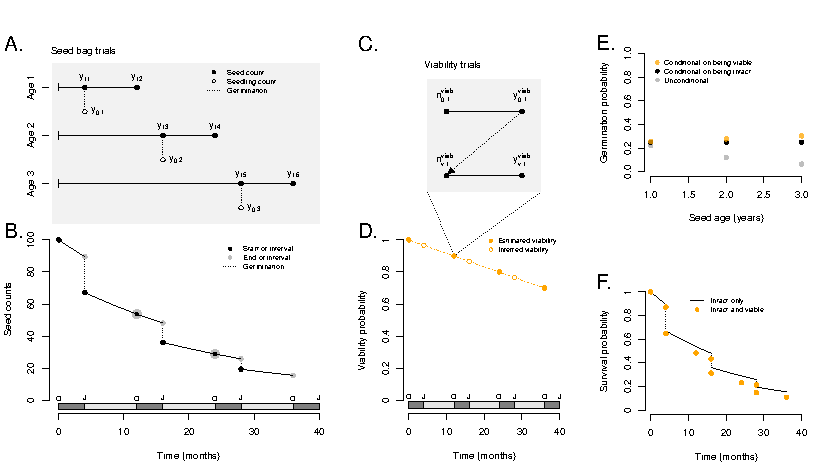
\includegraphics[width=\textwidth]{../../manuscript/figures/seed-bag-figure.pdf}  
    \caption{ Summary of the seed bag burial experiments and viability trials. \hl{Figure will be labeled as (A: seed bag trials , B: viability trials, C: germination probability, D: survival probability. }. (A) The gray panel contains a graphical representation of the seed bag trials. Seeds were buried at the start of each experiment (100 seeds in month 0). Seed bags were unearthed and intact seeds ($y_{\cdot \cdot}$) and germinants ($y_{\mathrm{g},\cdot}$ counted. The graph below the panel shows a hypothetical survival function associated with persistence of seeds in the soil seed bank. (B) The gray panel contains a graphical representation of the viability trials. Seeds were tested in two rounds; germination trials were performed and then some or all of the ungerminated seeds were tested for viability. The graph below the panel shows hypothetical data from a series of viability trials and the interpolated, inferred viabilities at times when viability was unobserved. (C) Age-specific germination probably is summarized in three ways. (D) The graph shows the survival function for persistence of seeds in the soil seed bank (black line) and the estimated discrete survival probabilities for persistence and viability of seeds (orange points). }
 \label{fig:seed-bag-experiments}
\end{figure}

The key pieces are Figure \ref{fig:seed-bag-experiments}, columns 1, 3, and 6 of Table \ref{tab:survival-functions} and columns 1 \& 3 in Table \ref{tab:structured-parameters}. Figure \ref{fig:seed-bag-experiments} illustrates the relationship between the seed bag burial experiment, viability trials, and survival/germination probabilities. Table \ref{tab:survival-functions} gives the mathematical relationship among the components of Figure \ref{fig:seed-bag-experiments}. Table \ref{tab:structured-parameters} translates the survival and germination components to parameters for the structured population model. I would to pare this down I would pare down Section \ref{section-1} to describe the experiment and reduce the tables to the relevant parameters, likely combining them into 1 table (top section being the survival functions, bottom section being the model parameters). I would keep the description of the full model and the viability models. I would move any discussion of how the models were constructed and DAGs to a separate document. I would reduce the section on translating estimated parameters to model parameters to generally describe how this was done and move the rest to a separate document. \hl{Note to self about how to turn this into Methods.} 

\subsection{Seedling and fruiting plant surveys in permanent plots}

To assess the survival of seedlings to fruiting plants, we use counts of seedlings and fruiting plants in 30 0.5 m$^2$ plots at 20 populations from 2006--\hl{2018} (\hl{Eckhart et al. 2011}). Seedlings and fruiting plants were counted in February and June, respectively. We observed counts of seedlings ($n_{ijk}$) and fruiting plants ($y_{ijk}$) in plot $i$, in population $j$, and in year $k$. Seedlings and fruiting plants in each plot are counted by a single person at each visit. 

Of more than 8000 observations, there were fewer seedlings than fruiting plants in approximately 5\% of observations; 50\% of these had 1 fewer seedling than fruiting plant. We assume that the data on fruiting plants is measured perfectly (i.e. we did not under- or over-count) because plants stand out from the background vegetation in June. We thus had to make an additional assumption about why we observed fewer seedlings than fruiting plants; this was necessary because we model seedling survival to fruiting as a binomial (\hl{see below}). There are at least two possible mechanisms that could contribute to observations in which the number of seedlings in a plot exceeds the number of fruiting plants observed later in the same year. An observer might miss a seedling that is present, or miss a seedling because germinants remained too small to observe at the February seedling census. 

\hl{For now, I excluded data that involved undercounting by filtering out those rows in the dataset. Alternatively, I could fit the model to data both by excluding or including the data and comparing the estimates. Future directions could include developing a model that relates our estimate of seedlings to the true number of seedlings in a plot because we sometimes observe more fruiting plants than seedlings (I had trouble developing such a model for the time being).}

\subsection{Surveys for fruits per plant \& seeds per fruit}

To assess the number of fruits per plant for \textit{C. xantiana}, we use data on counts of the number of fruits per plant at 20 populations (\cite{eckhart2011}). At each population, we made two sets of counts. First, from 2007--\hl{present}, we counted the number of fruits per plant on all plants in the 0.5m$^2$ permanent plots. Second, from 2006--\hl{present}, we counted the number of fruits per plant on plants that we sampled haphazardly across the site using throws of a 0.5m$^2$ grid. We chose to combine the datasets, one from plants in permanent plots and one from plants in haphazardly distributed plots, because the latter dataset sampled a broader distribution of plant sizes, and because it allowed us to estimate the distribution of fruit number per plant in years with relatively low survival in permanent plots. 

From 2006--2012, we counted the number of undamaged fruits on a plant. We then took the damaged fruits on a plant and visually stacked them end to end to estimate how many additional undamaged fruits that was equivalent to (e.g. two half fruits corresponded to one undamaged fruit). We used this as our count ($y^{TFE}_{ijk}$) of total fruit equivalents on plant $i$, in population $j$, and in year $k$. From 2013--\hl{present}, we counted and separately recorded the number of undamaged ($y^{UF}_{ijk}$) and damaged ($y^{DF}_{ijk}$) fruits on a plant plant. 

To assess the number of seeds per fruit for \textit{C. xantiana}, we use data on counts of the seeds per fruit of fruits that were haphazardly collected in 20 populations (\cite{eckhart2011}). In the field, we collected fruits that were undamaged. In the lab, we broke open the fruits to count the number of seeds per fruit. For each population in each year, we attempted to obtain 20-30 counts of seeds produced per undamaged fruit. The plants were outside permanent plots to avoid affecting seed input. We used these fruits to estimate the mean number of seeds produced by undamaged and damaged fruits.

From 2006--\hl{present}, we collected one undamaged fruit from each of 20-30 plants that were haphazardly collected across each population. We counted the number of seeds in the fruit ($y^{US}_{ijk}$), corresponding to fruit $i$, in population $j$, and in year $k$. From 2013--\hl{present}, we additionally collected a damaged fruit from the same plant whenever available. We counted the number of seeds in the fruit ($y^{DS}_{ijk}$), corresponding to fruit $i$, in population $j$, and in year $k$. 

\section{Model}

We use observational and experimental data from 20 populations of \textit{Clarkia xantiana} to estimate transition probabilities across the life cycle. We fit multilevel models to obtain population-specific estimates for belowground vital rates, and model year- and population-specific estimates for aboveground vital rates. Because we were interested in describing the life histories of individual populations, we built separate models for each population. Our general approach was to include a population-level mean as the top hierarchy, and have the next level be year-specific means drawn from the population mean. Although we used different likelihoods for different observations (e.g. binomial for seed bag experiments; Poisson for counts of seed per fruit), for a single population our approach can be summarized by the following model structure

\begin{align}
  \begin{split}
  [ \theta_j , \theta_0 , \sigma_j^2 , \varsigma^2 | y_{ij} ] &  \propto [ y_{ij} | \theta_j , \sigma^2_j] [ \theta_j | \theta_0 , \varsigma^2 ] [ \theta_0 ] [ \sigma^2_j] [ \varsigma^2].
  \end{split}
\end{align}

The distribution of the observations $y_{ij}$ is conditional on the year-specific parameters $\theta_j$ and $\sigma^2_j$. In turn, the year-specific parameter $\theta_j$ is conditional on the population-specific parameters $\theta_0$ and $ \varsigma^2$. All parameters found only on the right of conditional statements are also given priors ($\theta_0, \sigma^2_j, \varsigma^2$) In practice, we implemented this model by writing the upper levels of the model as Normal-Normal distributions; we thus drew year-specific means from a population-specific mean.

For each model, we include the expression for the posterior proportional to the joint distribution in \hl{Appendix: Joint Posterior}. Details about the choice of priors are give in \hl{Appendix: Priors}.

\subsection{Seed persistence and germination}

Describe full model at once; introduce model for germination then model for seed persistence as the product of absence of germination and destruction which combines the germination history and the deterministic survival function; then add the piece of estimating s0.

\begin{figure}[!h]
       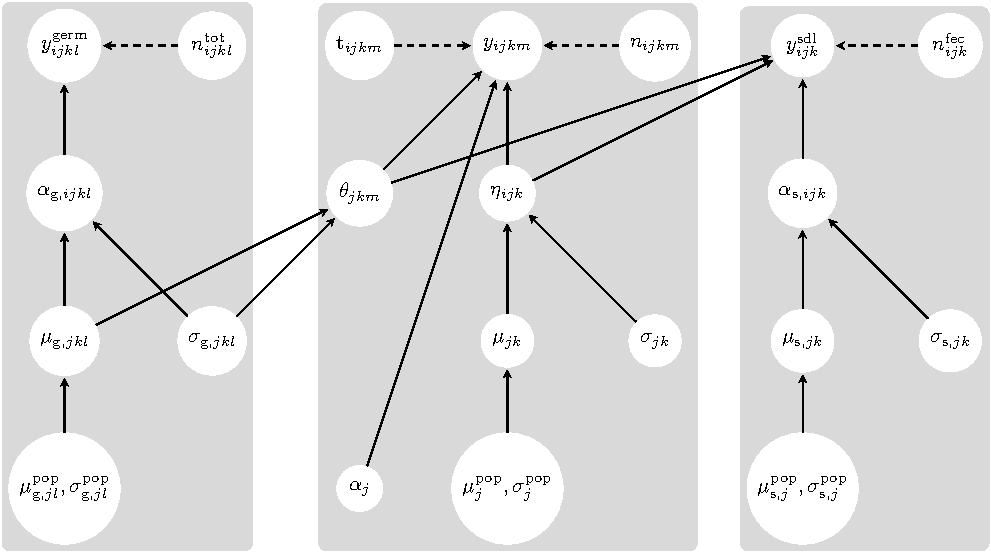
\includegraphics[width=\textwidth]{../../manuscript/figures/dag-seed-bag.pdf}  
    \caption{ Directed acyclic graphs for the full model. Models for each set of data are encapsulated in a gray box; links among the datasets are shown by arrows that cross over between boxes. Solid arrows depict the relationships among random variables, and dashed arrows depict the deterministic relationships. }
 \label{fig:dag-seed-bag}
\end{figure}

\subsection{Viability}

All data from viability trials is in the form of binomial trials: we have counts of seeds at the start and end of an experimental window of time. All models have the same structure for seeds in bag $i$ in population $j$ in experimental year $k$. If the number of seeds starting the trial (trials) is $n_{ijk}$ and the number of seeds at the end of the trial (successes) is $y_{ijk}$, we write a model that has a population-level mean and year-level means drawn from the population-level distribution. Broadly, this is two-level hierarchical model with a population-level mean, and year-level means drawn from the population-level distribution. The probability of success for each bag is drawn from this year- and population-level distribution. The model uses a binomial likelihood. 

\subsection{Seedling survival to fruiting}

\hl{Address missing years, low data years, pooling}

We estimated survival across all populations taking into account both temporal and between-population variability with the following model. We write a model that has a population-level mean and year-level means drawn from the population-level distribution. The probability of success (seedling survival to fruiting) for each plot is drawn from this year- and population-level distribution. The model has a binomial likelihood, and thus thus has a similar structure as the model for data on seed survival:
%
\begin{align}
  \begin{split}
 [  \bm{\alpha_S} , \bm{\mu_S} , \bm{\sigma_S} , \bm{\mu^\mathrm{pop}_S}, \bm{\sigma^\mathrm{pop}_S} | & \bm{y^{\mathrm{fruiting}}}  ] \propto \prod_{i=1}^{I}   \prod_{j=1}^{J}  \prod_{k=1}^{K} 
   \mathrm{binomial} ( y^{\mathrm{fruiting}}_{ijk} | n^\mathrm{seedling}_{ijk}, \mathrm{logit}^{-1}( \alpha_{S,ijk} ) ) 
   \\ & \times \mathrm{normal} ( \alpha_{S,ijk}  | \mu_{S,jk}, \sigma{_{S,jk} })
  \\ & \times \mathrm{normal} ( \mu_{S,jk}  | \mu^\mathrm{pop}_{S,j}, \sigma^\mathrm{pop}_{S,j} )
  \\ & \times \textrm{half-normal} ( \sigma_{S,jk} | 0,1)
  \\ & \times \mathrm{normal} ( \mu^\mathrm{pop}_{S,j} | 0 , 1000 ) \textrm{half-normal} ( \sigma^\mathrm{pop}_{S,j} | 0,1).
  \end{split}
\end{align}
%
We obtain the population- and population-by-year posterior distributions of seedling survival to fruiting ($\sigma$) by marginalization. We transform these posteriors to $[0,1]$ by taking the inverse logit; this transforms the parameters into the probability of success.

\begin{wrapfigure}[]{r}{0.25\textwidth}
       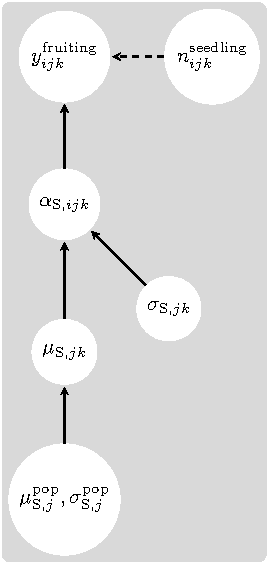
\includegraphics[scale=1]{../../manuscript/figures/dag-survival.pdf}  
    \caption{ Directed acyclic graphs for the model for seedling survival to fruiting. }
 \label{fig:dag-survival}
\end{wrapfigure}


\clearpage

\subsection{Fecundity: fruits per plant and seeds per fruit}


%Visual inspection of the data on total fruit equivalents (2006--2012) per plant suggests these counts are overdispersed. To assess what probability distribution to use when fitting this model, I fit a power model with an intercept to the mean and variance using the \textbf{nls} function in R, which returned an exponent of 1.85. The fit is close to quadratic which means a negative binomial is likely to be an appropriate distribution (\cite{linden2011}). 

We estimated fruits per plant across all populations taking into account both temporal and between-population variability with the following model. We constructed models with population-level mean and year-level means drawn from the population-level distribution. We used a Poisson likelihood to model the count data of fruits per plant. We modeled sampling uncertainty with a lognormal, which draws the true number of fruits (the $z$s) from a distribution with the median ($\mu$). Each combination of year and population is assigned its own sampling variance ($\sigma^2$). The general form of the model is the following: 
%
\begin{align}
  \begin{split}
  [ &  \bm{z} ,  \bm{\mu_{\mathrm{TF}}} ,  \bm{\sigma_{\mathrm{TF}}}^2 , ( \bm{\sigma^\mathrm{pop}_{\mathrm{TF}}})^2, \bm{\nu_{\mathrm{TF}}}  |  \bm{y^{\mathrm{TF}}} ]  \propto  \\  
 	     & \prod_{j=1}^{J} \prod_{i=1}^{N_1}  \prod_{k=1}^{K_1}  \mathrm{Poisson} ( y^\mathrm{TF}_{ijk} | z_{\mathrm{TF},ijk} )\ \mathrm{lognormal} ( z_{\mathrm{TF},ijk} | \mathrm{log}(\mu_{\mathrm{TF},jk}), \sigma^2_{\mathrm{TF},jk} )  \\
	     & \times \mathrm{lognormal} ( \mu_{\mathrm{TF},jk} | \mathrm{log}(\mathrm{g}(\nu_{\mathrm{TF},j}), (\sigma^\mathrm{pop}_{\mathrm{TF},j} )^2)  \\
	     & \times \mathrm{inverse\ gamma} ( \sigma^2_{\mathrm{TF},jk}  | 0.001, 0.001 ) \\
	     & \times \mathrm{gamma} (\nu_{\mathrm{TF},j} | 1 , 1)\  \mathrm{inverse\ gamma} ( (\sigma^\mathrm{pop}_{\mathrm{TF},j} )^2 | 0.001, 0.001 ) .
  \end{split}
\end{align}
%
We obtain the population- and population-by-year posterior distributions of fruits per plant ($F$) by marginalization. 

Estimating total fruit equivalents per plant required combining two types of data. First, I used counts of total fruit equivalents per plant from (2006-2012). I modeled these counts as observations ($z$s). Second, I used counts of undamaged and damaged fruits per plant from (2013-present). I separately modeled counts of each as observations to obtain estimates of undamaged and damaged fruits per plant. 

%Visual inspection of the data on undamaged fruits per plant (2013--2018) per plant suggests these counts are overdispersed. To assess what probability distribution to use when fitting this model, I fit a power model with an intercept to the mean and variance using the \textbf{nls} function in R, which returned an exponent of 1.97. The fit is close to quadratic which means a negative binomial i

\begin{figure}[!h]
       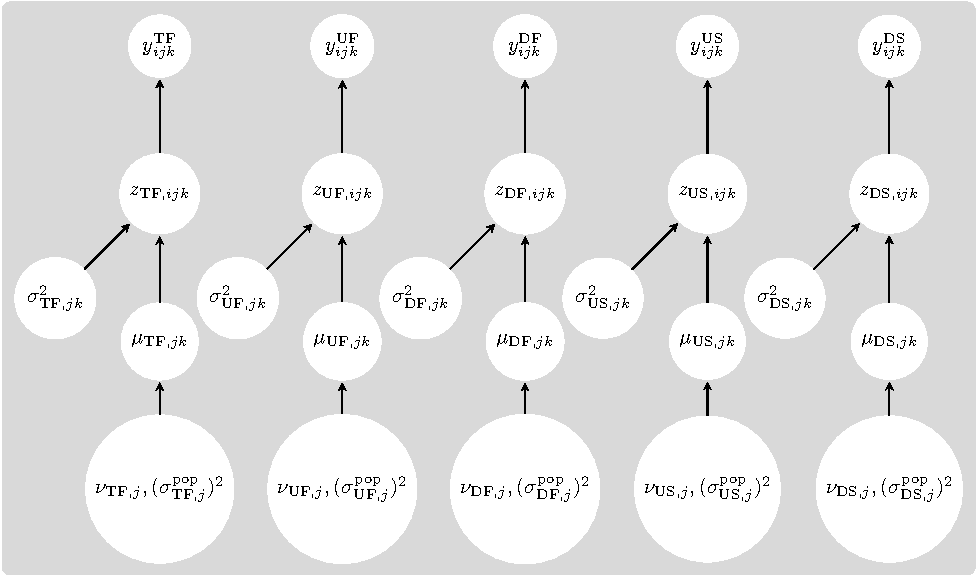
\includegraphics[scale=1]{../../manuscript/figures/dag-fecundity.pdf}  
    \caption{ Directed acyclic graphs for the models for fecundity. }
 \label{fig:dag-fecundity}
\end{figure}


%\hl{To assess what probability distribution to use when fitting this model,} I fit a power model with an intercept to the mean and variance using the \verb|nls| function in R, which returned an exponent of 1.38. The fit is greater than linear but less than quadratic which means that neither a Poisson nor negative binomial are likely to be entirely appropriate distributions for the data (\cite{linden2011}). I might try the parameterization in that reference but for now I am using the negative binomial because the data are overdispersed. 

We estimated seeds per fruit across all populations taking into account both temporal and between-population variability with the following model. We constructed models with population-level mean and year-level means drawn from the population-level distribution. We used a Poisson likelihood to model the count data of seeds per fruit. We modeled sampling uncertainty with a lognormal, which draws the true number of seeds (the $z$s) from a distribution with the median ($\mu$). Each combination of year and population is assigned its own sampling variance ($\sigma^2$). The general form of the model is the following: 
%
\begin{align}
  \begin{split}
  [ &  \bm{z} ,  \bm{\mu_{\mathrm{TF}}} ,  \bm{\sigma_{\mathrm{TF}}}^2 , ( \bm{\sigma^\mathrm{pop}_{\mathrm{TF}}})^2, \bm{\nu_{\mathrm{TF}}}  |  \bm{y^{\mathrm{TF}}} ]  \propto  \\  
 	     & \prod_{j=1}^{J} \prod_{i=1}^{N_1}  \prod_{k=1}^{K_1}  \mathrm{Poisson} ( y^\mathrm{TF}_{ijk} | z_{\mathrm{TF},ijk} )\ \mathrm{lognormal} ( z_{\mathrm{TF},ijk} | \mathrm{log}(\mu_{\mathrm{TF},jk}), \sigma^2_{\mathrm{TF},jk} )  \\
	     & \times \mathrm{lognormal} ( \mu_{\mathrm{TF},jk} | \mathrm{log}(\mathrm{g}(\nu_{\mathrm{TF},j}), (\sigma^\mathrm{pop}_{\mathrm{TF},j} )^2)  \\
	     & \times \mathrm{inverse\ gamma} ( \sigma^2_{\mathrm{TF},jk}  | 0.001, 0.001 ) \\
	     & \times \mathrm{gamma} (\nu_{\mathrm{TF},j} | 1 , 1)\  \mathrm{inverse\ gamma} ( (\sigma^\mathrm{pop}_{\mathrm{TF},j} )^2 | 0.001, 0.001 ) .
  \end{split}
\end{align}
%
We obtain the population- and population-by-year posterior distributions of seeds per fruit ($\phi$) by marginalization. 

First, I used counts of seeds per undamaged fruit (2006-present). I modeled these counts as observations ($z$s). Second, I used counts of seeds from damaged fruits per plant from (2013-present). I separately modeled counts of each as observations to obtain estimates of seeds per damaged fruit.

\section{Computing vital rates}

General summary should cover link of parameter estimates from observational and experimental data to structured model parameters. Key issues to address are different kinds of data collection in different years, as well as combining datasets to get a coherent estimate for a parameter (correct support).

Use model checking and compare outputs to look at effect of accounting for viability in belowground rates, and understand that certain years in aboveground rates had no data in permanent plots and were thus more strongly pooled. 

\subsection{Belowground vital rates}

Describe calculating persistence + persistence/viability.
Then describe linking these to the structured parameters

\singlespace
%
\begin{center}
\captionof{table}{ Seed persistence and viability in the soil seed bank } \label{tab:survival-functions} 
 \begin{tabularx}{11cm}{l  | c | l    } 
  \multicolumn{1}{ c | }{  } & 
  \multicolumn{1}{ c |  }{ Persistence } & 
   \multicolumn{1}{ c  }{ Persistence \& viability } \\ 
 \hline
 \hline
 \multicolumn{1}{ l }{ Time $(x_i)$ } & 
\multicolumn{1}{ | c | }{ $S(x_i)$ } & 
 \multicolumn{1}{ c }{ $S(x_i)$ } \\
 \hline

 $\mathrm{Oct_0}$ & $\theta_0$ & $\phi_0 =  \theta_0$  \\

  $\mathrm{Jan_{1,total}}$ & $\theta_1$ & $\phi_1 = \theta_1 (\gamma_1 + (1-\gamma_1) \nu^{1/3}_1 ) $   \\

  $\mathrm{Jan_{1,intact}}$ & $\theta_2$ & $\phi_2 = \theta_2 \nu^{1/3}_1$  \\

   $\mathrm{Oct}_1$ & $\theta_3$ & $\phi_3 = \theta_3 \nu_1$  \\

  $\mathrm{Jan_{2,total}}$ & $\theta_4$ & $\phi_4 = \theta_4 (\gamma_2 + (1-\gamma_2) \nu_1 (\nu_2 / \nu_1 )^{1/3}) $ \\

  $\mathrm{Jan_{2,intact}}$ & $\theta_5$ & $\phi_5 = \theta_5 \nu_1 (\nu_2 / \nu_1)^{1/3}$  \\
 
   $\mathrm{Oct}_2$ &  $\theta_6$ & $\phi_6 = \theta_6  \nu_2 $  \\
   
  $\mathrm{Jan_{3,total}}$ & $\theta_{7}$  & $\phi_7 = \theta_7 (\gamma_3 + (1-\gamma_3) \nu_2 (\nu_3 / \nu_2 )^{1/3})   $  \\

  $\mathrm{Jan_{3,intact}}$ & $\theta_{8}$ & $\phi_8 = \theta_8 \nu_2 (\nu_3 / \nu_2 )^{1/3}$   \\
 
   $\mathrm{Oct}_3$ &  $\theta_{9}$  & $\phi_9 = \theta_9 \nu_3$ \\
 
  \hline
\end{tabularx}
\end{center}
%
\doublespace


The survival function for viable seeds ($\phi$) is composed of estimates of persistence over time ($\theta_\cdot$), estimates of viability ($\nu_\cdot$), and estimates of germination conditional on persistence ($\gamma_\cdot$). We used the survival function and germination probabilities to define the parameters in the structured population model for \textit{Clarkia xantiana} ssp. \textit{xantiana}. Table \ref{tab:structured-parameters} defines the age-specific germination probabilities and survival probabilities for the Leslie matrix in \hl{Eckhart et al. 2011} in terms of the survival function (Table \ref{tab:survival-functions}) and germination probabilities. 
%
\singlespace%
\begin{center}
\captionof{table}{ Structured model parameters conditional on persistence and viability } \label{tab:structured-parameters} 
 \begin{tabularx}{4.5cm}{c c } 
 \hline
 \hline
  \multicolumn{1}{ c }{Parameter} & 
   \multicolumn{1}{ c }{ Probability }  \\
\hline

 $g_1$  & $  \gamma_1  / \phi_1 $ \\

 $g_2$ & $  \gamma_2  / \phi_4 $ \\

 $g_3$ & $  \gamma_3  / \phi_7 $ \\

 \hline

 $s_1$ & $ \phi_1$ \\

 $s_2$ &  $ \phi_3 / \phi_2 $  \\

$s_3$ & $  \phi_4 / \phi_3  $ \\
 
$s_4$ &  $  \phi_6 / \phi_5 $ \\
   
$s_5$ &  $  \phi_7 / \phi_6  $  \\
 
 $s_6$ &  $  \phi_9 / \phi_8  $  \\
 
  \hline
\end{tabularx}
\end{center}
\doublespace

Figure \ref{fig:seed-bag-experiments}C illustrates the relationship among the pieces discussed here. Estimates of germination from the seed bag experiment correspond to the probability of germination conditional on persistence (e.g. $\gamma_1$). Multiplying these estimates by the probability of persistence in January before germination gives the unconditional probability of germination (e.g. $\theta_1 \times \gamma_1$). Finally, the probability of germination conditional on viability is estimated by incorporating loss of viability into the survival function (e.g. $\gamma_1 / \phi_1$).

We tested the viability of seeds in October, and were thus able to estimate the proportion of viable seeds (Figure \ref{fig:seed-bag-experiments}B; filled points). We further inferred the viability of intact seeds in January by assuming that seeds lost viability at a constant rate (exponential decay). Further, we interpolated between estimates by assuming that viability changed at a constant rate between years, and that all seeds were viable at the start of the experiment (Figure \ref{fig:seed-bag-experiments}B; open points).

\subsection{Aboveground vital rates}

Describe using the posteriors to calculate ratio of and get TFE equivalents in later years. 

\clearpage
\newpage




\clearpage
%%%%%%%%%%%%%%%%%%%%%%%%%%%%%%%%%%%%%%%%%%%%%%%%%%%%
% BIBLIOGRAPHY
%%%%%%%%%%%%%%%%%%%%%%%%%%%%%%%%%%%%%%%%%%%%%%%%%%%%
\bibliographystyle{/Users/gregor/Dropbox/bibliography/styleFiles/ecology} 
\bibliography{/Users/gregor/Dropbox/bibliography/chapter-1}

\end{document}